\documentclass[10pt,a4paper]{article}
\usepackage[preprint]{neurips_2025}
\usepackage[utf8]{inputenc}
\usepackage[T1]{fontenc}
\usepackage[vietnamese]{babel}
\usepackage{geometry}
\geometry{a4paper, top=1.5cm, bottom=1.5cm, left=1.5cm, right=1.5cm}
\usepackage{graphicx}
\usepackage{enumitem}
\usepackage{amsmath}
\usepackage{amsfonts}
\usepackage{titlesec}
\usepackage{caption}
\usepackage{float}
\usepackage{hyperref}
% \titlespacing*{\section}{0pt}{1.5ex plus 1ex minus .2ex}{0.8ex plus .2ex}
% \titlespacing*{\subsection}{0pt}{1ex plus 1ex minus .2ex}{0.5ex plus .2ex}
\setlength{\columnsep}{0.6cm}
\title{
  Từ Rò rỉ Nhu cầu đến Ma sát Tồn kho: \\
  Phân tích Dữ liệu và Dự báo Doanh thu cho Thương mại Điện tử Thời trang
}

\author{
  HTTPs \\
  Datathon 2026 -- The Gridbreaker
}
\begin{document}
\maketitle
\begin{abstract}
  Báo cáo này phân tích bộ dữ liệu mô phỏng hoạt động của một doanh nghiệp thương mại điện tử thời trang tại Việt Nam, với mục tiêu phát hiện các điểm nghẽn ảnh hưởng đến tăng trưởng doanh thu và xây dựng mô hình dự báo doanh thu có khả năng giải thích. Dữ liệu bao gồm nhiều lớp thông tin, từ dữ liệu khách hàng, sản phẩm, đơn hàng, thanh toán, trả hàng, khuyến mãi, tồn kho, lưu lượng truy cập website đến chuỗi doanh thu theo ngày. Trọng tâm phân tích của chúng tôi được chia thành hai hướng chính: \textit{rò rỉ nhu cầu} ở phía khách hàng, thể hiện qua hành vi không chuyển đổi, không mua lại hoặc suy giảm giá trị theo thời gian; và \textit{ma sát tồn kho} ở phía vận hành, thể hiện qua tình trạng hết hàng, dư hàng và khả năng đáp ứng nhu cầu chưa tối ưu.

  Thông qua các phương pháp trực quan hoá dữ liệu, phân tích cohort, phân khúc khách hàng, chẩn đoán hiệu quả tồn kho và liên kết giữa lưu lượng truy cập với doanh thu, báo cáo chuyển hoá các mẫu hình dữ liệu thành các insight kinh doanh có thể hành động. Bên cạnh đó, chúng tôi xây dựng một pipeline dự báo doanh thu theo chuỗi thời gian, sử dụng các đặc trưng được tạo hoàn toàn từ bộ dữ liệu được cung cấp, đồng thời kiểm soát rò rỉ dữ liệu và đảm bảo khả năng tái lập kết quả. Kết quả phân tích và mô hình hoá cho thấy việc kết hợp giữa phân tích mô tả, chẩn đoán, dự báo và đề xuất hành động có thể hỗ trợ doanh nghiệp tối ưu phân bổ tồn kho, điều chỉnh chiến lược khuyến mãi, cải thiện giữ chân khách hàng và nâng cao độ chính xác trong lập kế hoạch doanh thu.
\end{abstract}
\newpage
\section{Trực quan hóa và phân tích}

\subsection{Từ rò rỉ nhu cầu đến ma sát tồn kho}

Thay vì xem tăng trưởng doanh thu chỉ như một bài toán tăng traffic hay tăng tồn kho, chúng tôi đặt câu hỏi ở cấp hệ thống: \textbf{nhu cầu được tạo ra có được chuyển hóa thành doanh thu đúng thời điểm hay không?} Từ đó, phân tích được chia thành hai lớp liên kết: \textit{demand-side leakage} ở hành trình khách hàng và \textit{supply-side friction} ở khả năng đáp ứng sản phẩm. Cách tiếp cận này cho phép nối trực tiếp các mẫu hình trong dữ liệu với quyết định kinh doanh: giữ chân khách hàng, ưu tiên danh mục hàng hóa, và điều phối tồn kho theo tín hiệu nhu cầu.

\subsection{Demand-side: khách hàng vào hệ thống nhưng chưa được kích hoạt đủ sâu}

\begin{figure}[h]
  \centering
  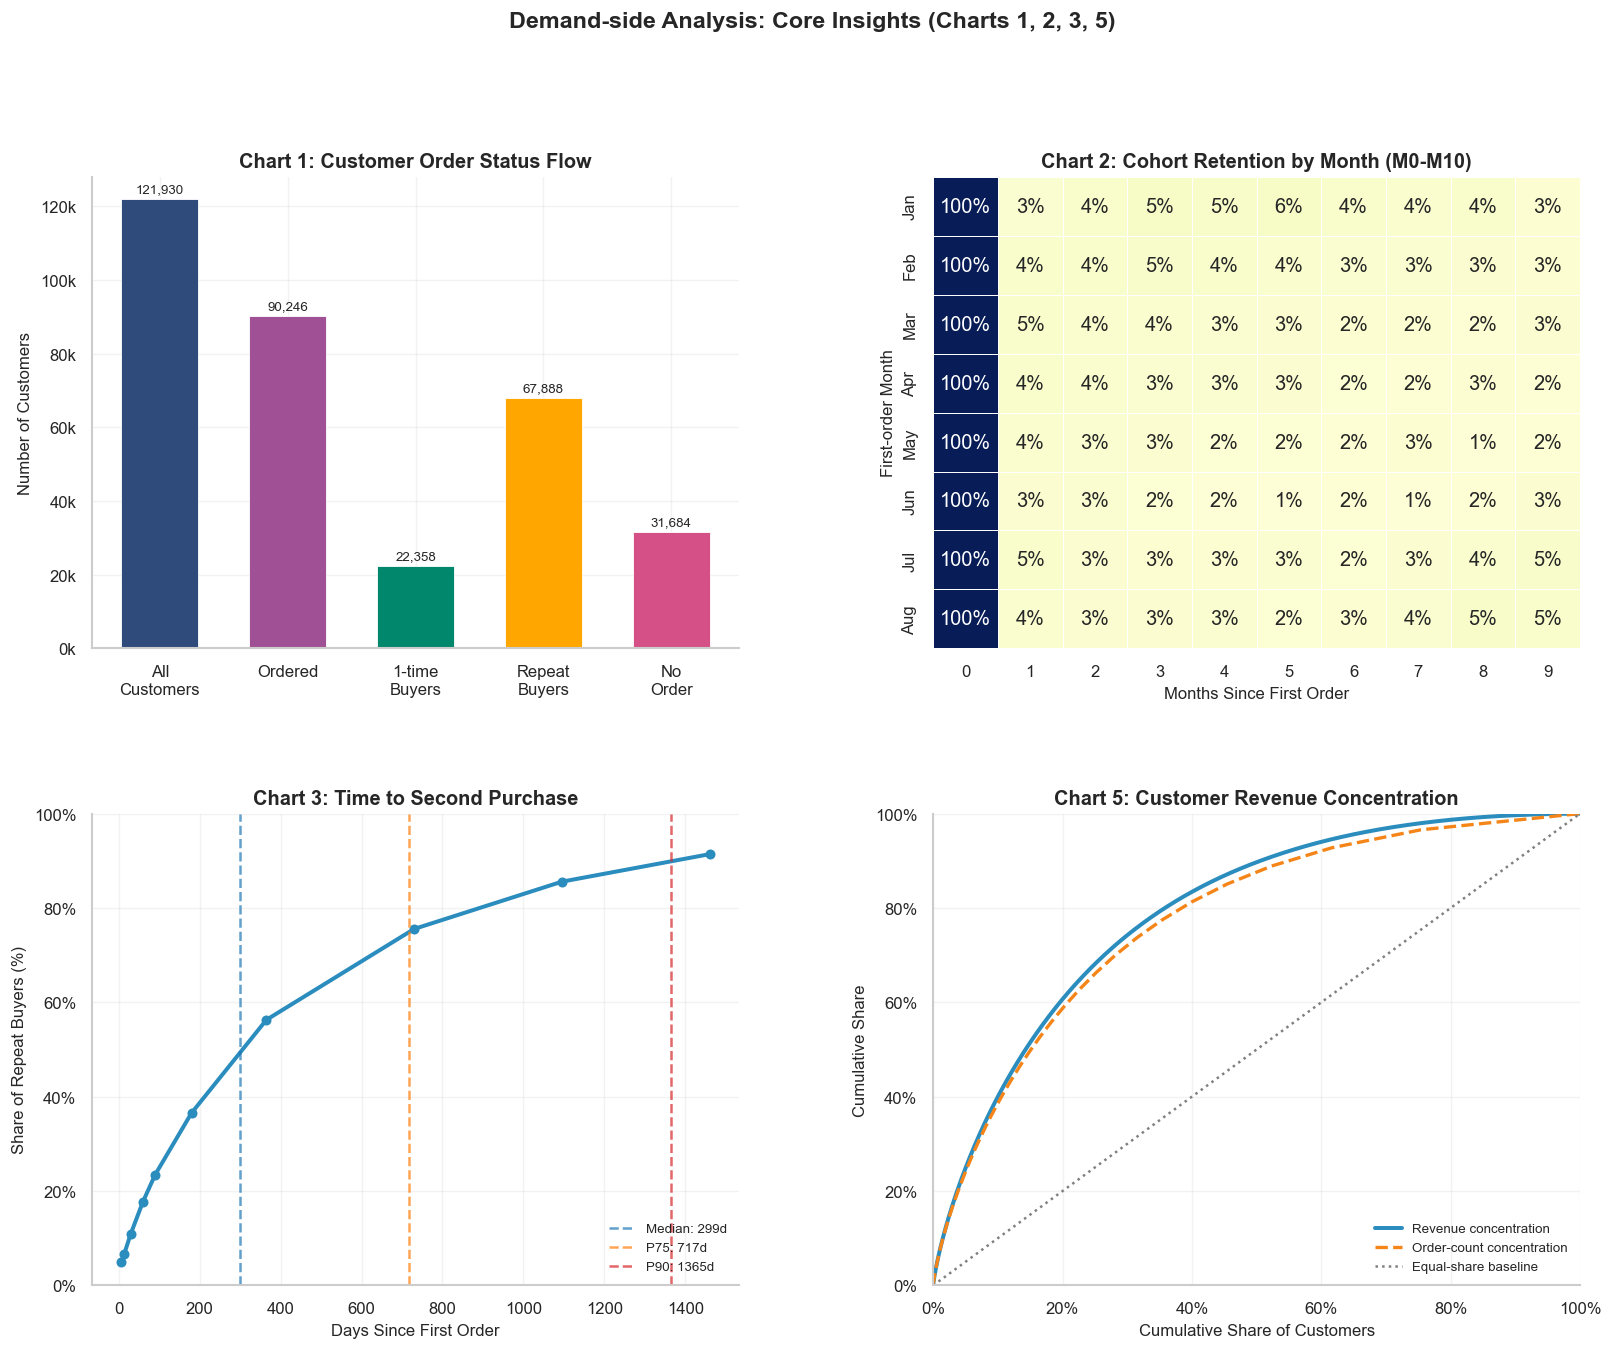
\includegraphics[width=0.98\linewidth]{demand.png}
  \caption{Demand-side analysis: phễu chuyển đổi, retention theo cohort, thời gian đến lần mua thứ hai, và mức độ tập trung doanh thu.}
  \label{fig:demand_composite}
\end{figure}

Hình~\ref{fig:demand_composite} cho thấy điểm nghẽn demand không nằm ở việc thiếu người dùng đầu vào, mà nằm ở \textbf{khả năng chuyển hóa và duy trì nhu cầu sau khi khách đã vào hệ thống}. Trong tổng số 121{,}930 khách hàng, có 90{,}246 khách từng đặt hàng, tương ứng khoảng 74.0\%; ngược lại, 31{,}684 khách chưa tạo đơn nào, tức khoảng 26.0\% tệp khách hàng vẫn chưa được kích hoạt. Ở lớp sau đơn đầu tiên, nhóm mua một lần chiếm 22{,}358 khách, trong khi 67{,}888 khách có hành vi mua lặp lại. Điều này cho thấy rò rỉ không chỉ xảy ra trước đơn hàng đầu tiên, mà còn xuất hiện ở giai đoạn biến người mua lần đầu thành khách hàng quay lại.

Phân tích cohort bổ sung thêm một lớp chẩn đoán quan trọng: retention sau tháng đầu giảm rất nhanh và duy trì ở mức thấp trong các tháng sau, nhưng mức giảm không đồng nhất giữa các cohort. Nói cách khác, khách hàng không biến mất theo cùng một nhịp; họ chịu ảnh hưởng bởi thời điểm gia nhập, mùa vụ và trải nghiệm sau mua. Vì vậy, nếu chỉ đo churn bằng một ngưỡng cố định như 30 hoặc 90 ngày, doanh nghiệp có thể đánh giá sai chất lượng khách hàng và cắt nhầm ngân sách CRM cho những nhóm thực ra vẫn có khả năng quay lại.

Biểu đồ thời gian đến lần mua thứ hai củng cố nhận định này: một phần lớn khách hàng quay lại muộn hơn khung đo ngắn hạn. Do đó, vấn đề không nên được diễn giải đơn giản là ``khách đã rời bỏ'', mà là \textbf{doanh nghiệp chưa can thiệp đúng thời điểm trong chu kỳ mua lại}. Đồng thời, đường tập trung doanh thu cho thấy doanh thu phụ thuộc mạnh vào một nhóm khách hàng giá trị cao, khiến tăng trưởng trở nên nhạy cảm nếu nhóm này giảm tần suất mua.

Từ các bằng chứng trên, ưu tiên 90 ngày cho demand-side là: \textbf{(i)} tăng chuyển đổi từ đăng ký sang đơn đầu bằng ưu đãi kích hoạt hoặc onboarding cá nhân hóa; \textbf{(ii)} thiết kế CRM theo cohort và theo thời gian từ đơn gần nhất thay vì gửi đại trà; \textbf{(iii)} bảo vệ nhóm khách hàng mid-high và top bằng ưu đãi giữ chân có điều kiện. Các KPI cần theo dõi hàng tuần gồm: signup-to-order rate, first-to-second-order rate, median days to second purchase, repeat rate theo cohort, và tỷ trọng doanh thu từ nhóm khách hàng giá trị cao.

\subsection{Supply-side: không thiếu hàng tổng thể, mà lệch pha giữa tồn kho và nhu cầu}

\begin{figure}[h]
  \centering
  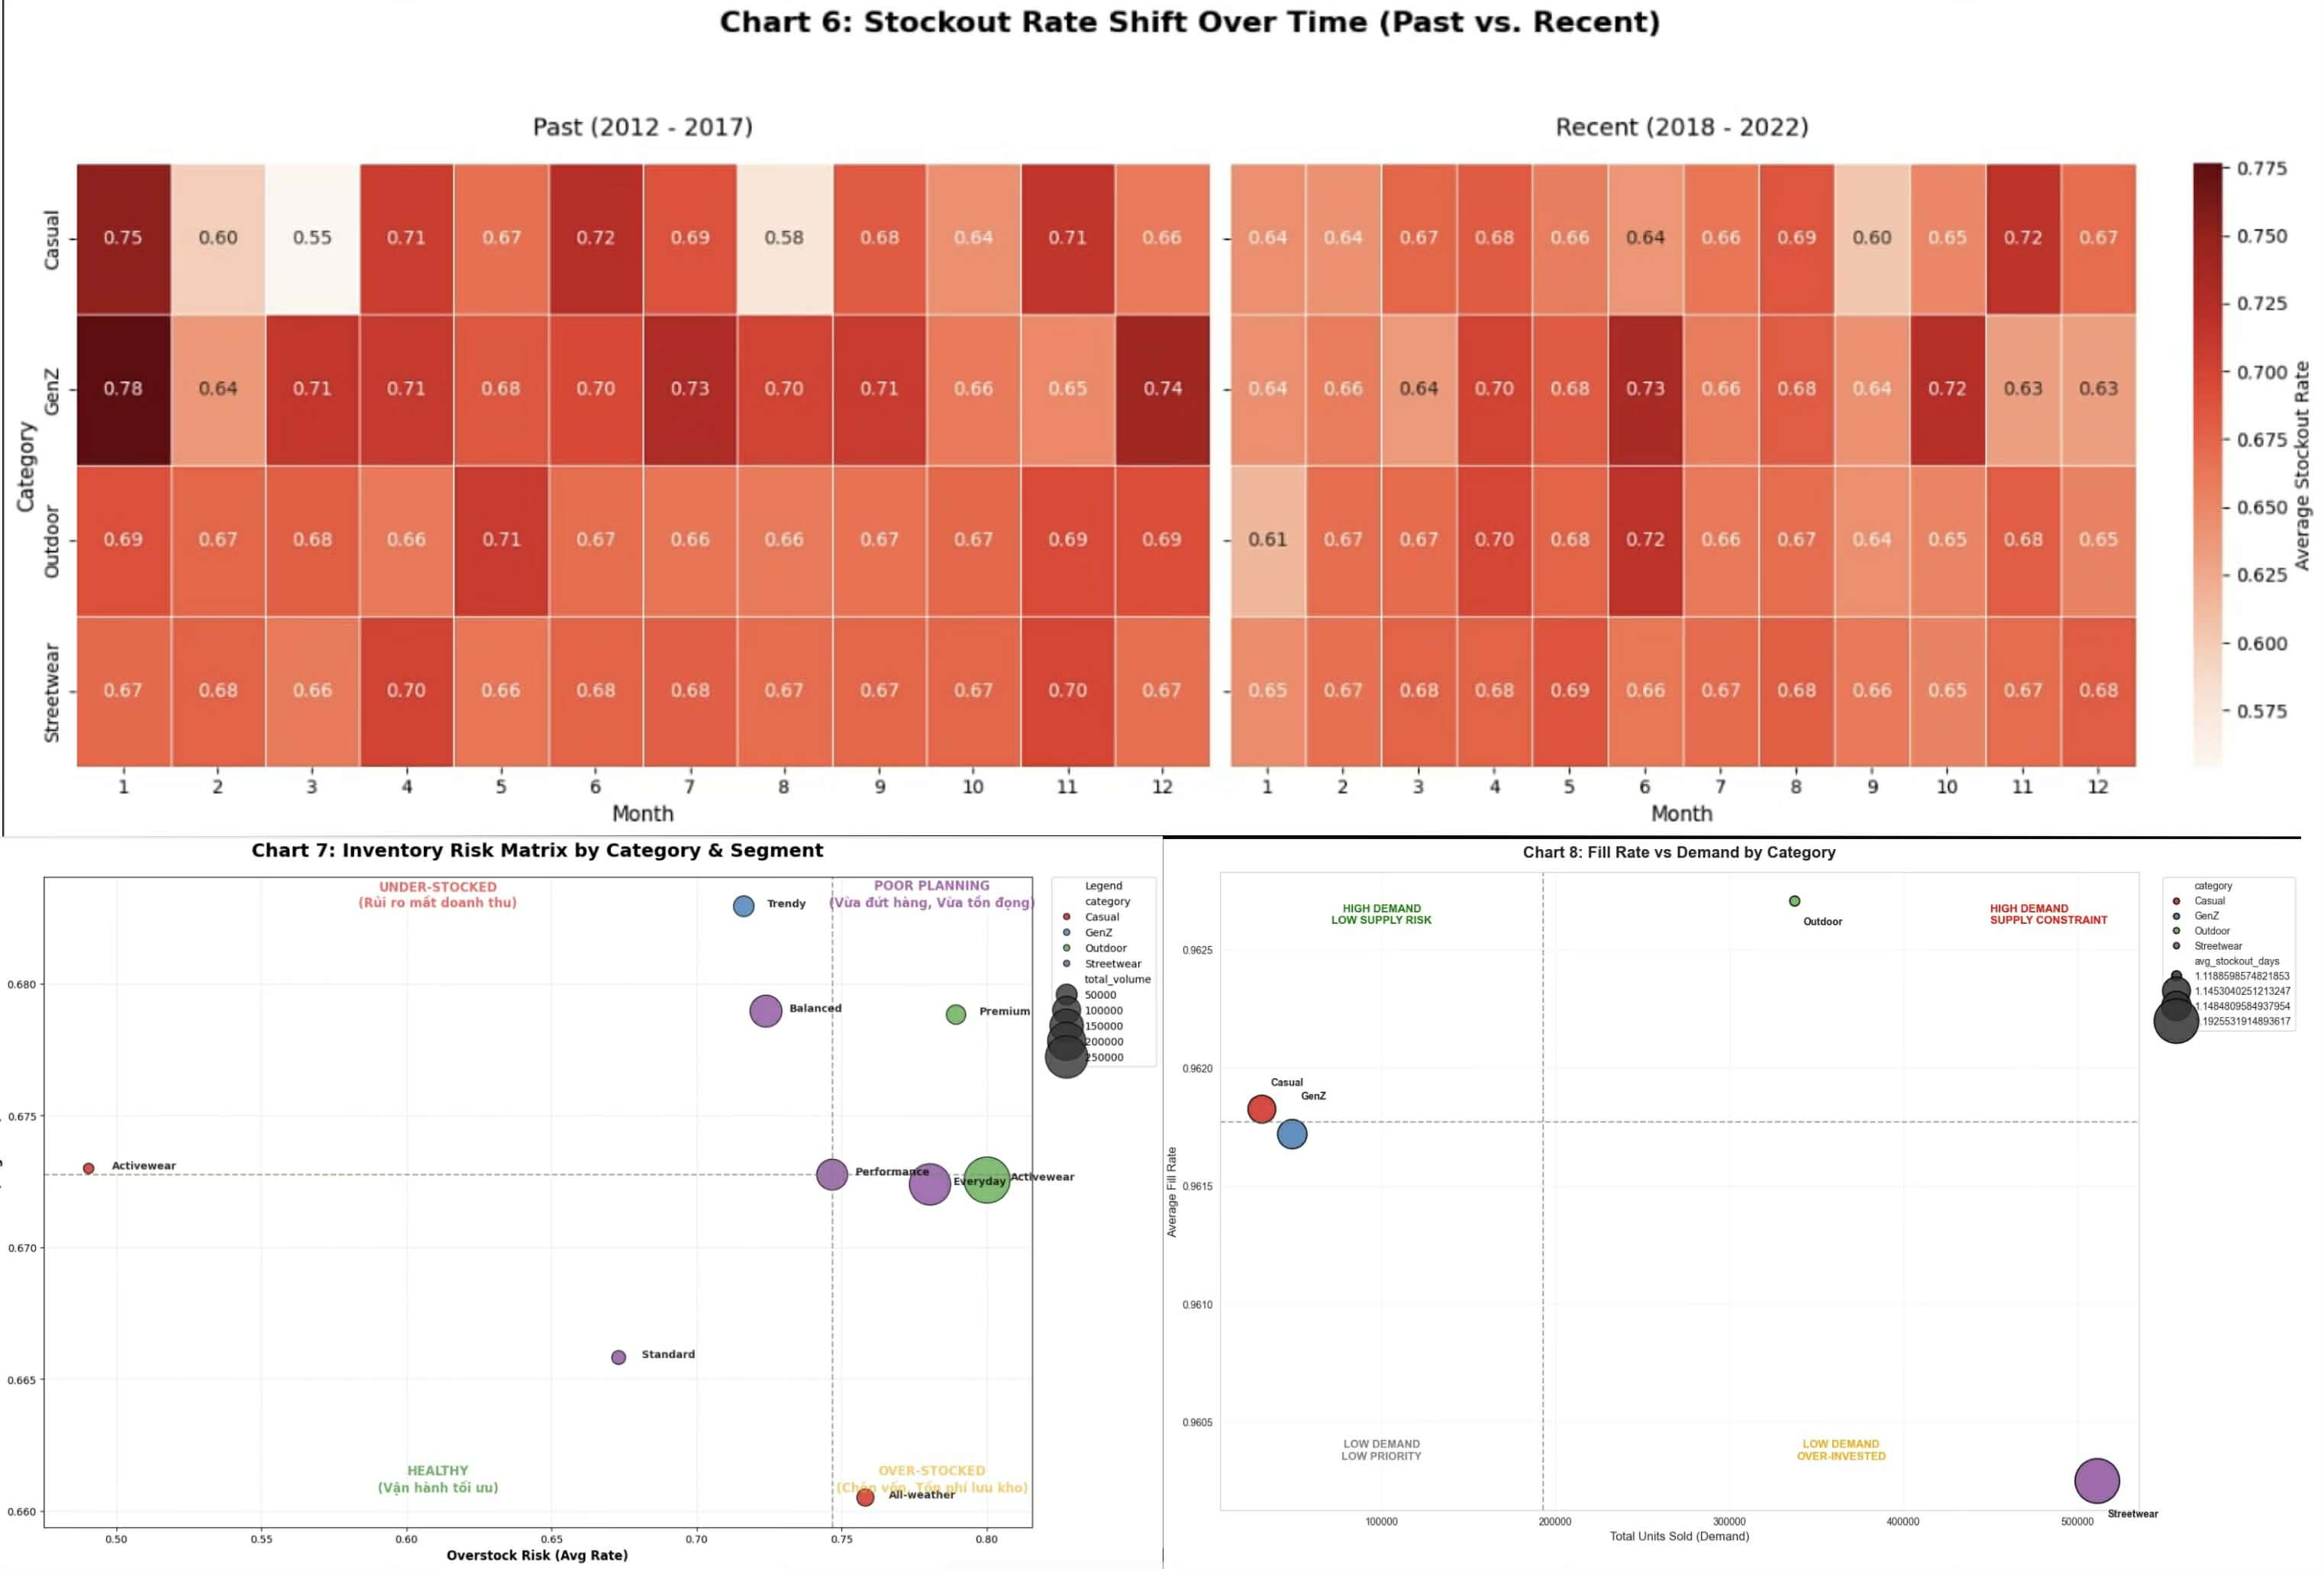
\includegraphics[width=0.96\linewidth]{supply.png}
  \caption{Supply-side analysis: stockout theo thời gian, ma trận rủi ro tồn kho, và hiệu quả đáp ứng theo danh mục.}
  \label{fig:supply_composite}
\end{figure}

Nếu demand-side cho thấy doanh nghiệp đang bỏ lỡ một phần nhu cầu từ khách hàng, thì Hình~\ref{fig:supply_composite} cho thấy một nguyên nhân vận hành tương ứng: \textbf{tồn kho không được phân bổ đúng theo nơi nhu cầu phát sinh}. Stockout xuất hiện lặp lại qua nhiều tháng và không phân bố ngẫu nhiên, cho thấy đây không phải nhiễu cục bộ mà là vấn đề có tính hệ thống trong dự báo và bổ sung hàng. Đáng chú ý, sự khác biệt giữa giai đoạn cũ và giai đoạn gần đây cho thấy rủi ro tồn kho có yếu tố mùa vụ và thay đổi theo thời gian, vì vậy chính sách nhập hàng cố định theo trung bình lịch sử sẽ khó bắt kịp nhu cầu thực tế.

Ma trận rủi ro tồn kho cho thấy hai dạng lãng phí xảy ra đồng thời: một số nhóm hàng bị overstock, làm khóa vốn và tăng chi phí lưu kho; trong khi một số nhóm khác lại under-stock hoặc stockout, làm mất cơ hội doanh thu. Đây là dấu hiệu của \textbf{mismatch trong product mix}: doanh nghiệp có hàng, nhưng không phải đúng danh mục, đúng thời điểm và đúng mức nhu cầu. Vì thế, việc tăng tổng lượng hàng nhập chưa chắc giải quyết vấn đề; hành động quan trọng hơn là tái phân bổ nguồn lực theo danh mục và theo tín hiệu bán thực tế.

Ở cấp danh mục, vùng ưu tiên không nên được xác định chỉ bằng stockout cao nhất tuyệt đối, mà bằng tổ hợp giữa quy mô bán lớn và khả năng đáp ứng chưa tương xứng. Streetwear là điểm rủi ro nổi bật nhất về mặt cơ hội doanh thu: đạt \textbf{511{,}467 units sold}, chiếm \textbf{55.1\%} tổng lượng bán quan sát được, đồng thời có stockout trung bình cao nhất, khoảng \textbf{1.19 ngày/tháng}. Khi dùng \textit{units sold} làm proxy cho nhu cầu quan sát được và tính \textit{fill rate} có trọng số theo lượng bán, fill rate của Streetwear đạt khoảng \textbf{94.97\%}; mức này không phải thấp nhất tuyệt đối, nhưng do quy mô bán rất lớn nên tạo ra \textit{lost units proxy} cao nhất, khoảng \textbf{43{,}978} đơn vị, tương đương \textbf{49.23\%} tổng lost units proxy. Streetwear bán nhiều hơn Outdoor khoảng \textbf{1.52 lần}. Vì vậy, Streetwear vẫn nên là danh mục ưu tiên bổ sung hàng trong ngắn hạn, trong khi các danh mục overstock cần giảm nhập, bundle hoặc markdown có mục tiêu. KPI vận hành nên theo dõi gồm fill rate theo danh mục, stockout days, sell-through rate và lost units proxy.

\subsection{Hàm ý kinh doanh: đồng bộ demand và supply}

Hai lớp phân tích trên dẫn đến cùng một kết luận: doanh nghiệp không chỉ mất doanh thu vì thiếu khách hàng, cũng không chỉ vì thiếu hàng hóa. Vấn đề cốt lõi là \textbf{thiếu cơ chế đồng bộ giữa tín hiệu nhu cầu và quyết định đáp ứng}. Demand-side tạo ra khách hàng và ý định mua, nhưng supply-side chưa luôn đặt đúng sản phẩm vào đúng thời điểm. Khi hai hệ thống vận hành tách rời, doanh nghiệp vừa tốn chi phí acquisition và CRM, vừa không tận dụng hết nhu cầu đã tạo ra.

Chiến lược đề xuất là xây dựng một vòng điều phối khép kín: tín hiệu từ phễu khách hàng, cohort retention và thời gian mua lại được đưa vào dự báo nhu cầu theo danh mục; sau đó kế hoạch tồn kho được điều chỉnh theo fill rate, stockout và sell-through. Với cách này, marketing không chỉ tối ưu lượng khách vào, mà còn phối hợp với vận hành để đảm bảo những danh mục khách có khả năng mua cao luôn sẵn hàng. Ngược lại, tồn kho không chỉ được tối ưu theo mức bán quá khứ, mà còn theo cơ hội doanh thu tương lai.

Tóm lại, tăng trưởng bền vững nên được triển khai theo ba ưu tiên: \textbf{giảm rò rỉ đầu phễu}, \textbf{rút ngắn chu kỳ mua lại}, và \textbf{tái phân bổ tồn kho theo nhu cầu thực tế}. Đây là hướng hành động vừa có thể đo lường ngắn hạn bằng conversion, repeat rate và fill rate, vừa tạo nền tảng dài hạn cho mô hình dự báo doanh thu ở phần tiếp theo.
\section{Mô hình dự đoán}
\subsection{Đặt vấn đề \& Thách thức}
Bài toán yêu cầu dự báo doanh thu và giá vốn (COGS) trong khung thời gian cực dài (18 tháng - 548 ngày) mang đến 3 rào cản chí tử:
\begin{itemize}[leftmargin=*, nosep]
  \item \textbf{Cấm kỵ biến trễ (Lag-free):} Khung thời gian 548 ngày khiến các biến tự hồi quy ($y_{t-n}$) mất tác dụng, nguy cơ tích lũy sai số (error accumulation) rất lớn.
  \item \textbf{Đứt gãy cấu trúc (Regime Drift):} Mức nền doanh thu thay đổi đột ngột sau đại dịch (2020-2022) (Chi tiết tại phụ lục \ref{app: Revenue, COGS, Profit plot}).
  \item \textbf{Biến động cục bộ:} Biên độ dao động cực lớn tại các sự kiện Lễ/Tết và ngày siêu sale (Black Friday).
\end{itemize}
\subsection{Khai phá Đặc trưng (Feature Engineering)}
Để triệt tiêu sự phụ thuộc vào biến trễ, mô hình tiếp cận theo hướng \textbf{Direct Forecasting}, xây dựng tọa độ thời gian tuyệt đối\citep{taylor2018forecasting}:
\begin{itemize}[leftmargin=*, nosep]
  \item \textbf{Đặc trưng Fourier (Cyclical Encoding):} Chuyển đổi \textit{Day of Year, Day of Month, Day of Week} thành các sóng lượng giác ($\sin, \cos$). Giúp mô hình nội suy hoàn hảo bản đồ mùa vụ.
  \item \textbf{Sự kiện \& Tiệm cận (Proximity):} Tính khoảng cách đếm ngược/tiến đến các mốc sự kiện (Tet distance, End of month) giúp dự báo chính xác các đỉnh dư âm và bắt nhịp sale.
\end{itemize}
Mô hình tuân thủ kiểm định khắt khe bằng \textbf{3 Temporal Folds} (Chi tiết tại Phụ lục \ref{app: ML Anti-Leakage Strategy}).
\subsection{Kiến trúc Ensemble Đa tầng}
Hệ thống sử dụng luồng phân tầng (Tiered Ensemble) kết hợp đa thuật toán để triệt tiêu phương sai và bình ổn dư lượng \citep{sagi2018ensemble} (Diagram pipeline chi tiết tại phụ lục \ref{app:ML})
\subsubsection{Tier 1: Custom Seasonal Blending}
Nhằm sửa lỗi margin của mô hình \textbf{LightGBM Generalist} \citep{ke2017lightgbm}, 4 mô hình \textbf{Q-Specialists} (chuyên gia theo Quý) được khởi tạo độc lập. Chiến lược \textit{Heuristic Blending} được áp dụng: Hệ số pha trộn chuyên gia $\alpha$ được thiết lập ở mức $0.6$ cho các quý ổn định (Q1, Q2, Q4). Riêng Q3 có độ lệch margin lớn, $\alpha_3 = 1.0$ được kích hoạt nhằm ép đường dự báo về đúng quỹ đạo (Chi tiết tại Phụ lục \ref{app: ML blending Logic}).
\subsubsection{Tier 2: Multi-family Integration}
Kết quả Blending ở Tier 1 được kết hợp song song với 2 hệ tư tưởng khác biệt để bình ổn rủi ro:
\begin{itemize}[leftmargin=*, nosep]
  \item \textbf{Ridge Regression\citep{hoerl1970ridge}:} Bắt Global Linear Trend ổn định.
  \item \textbf{Prophet\citep{taylor2018forecasting}:} Chuyên biệt xử lý Post-Regime (train từ 2020).
\end{itemize}
Trọng số kết hợp cuối cùng được tối ưu bằng Non-Negative Least Squares (NNLS) (chi tiết tại phụ lục \ref{app: ML NNLS}).

\subsection{Động lực Dự báo (Model Explainability)}
Sử dụng Feature Importance (\textit{Split Count}) của mô hình lõi LightGBM để minh bạch hóa động lực học của thuật toán.

\begin{figure}[H]
  \centering
  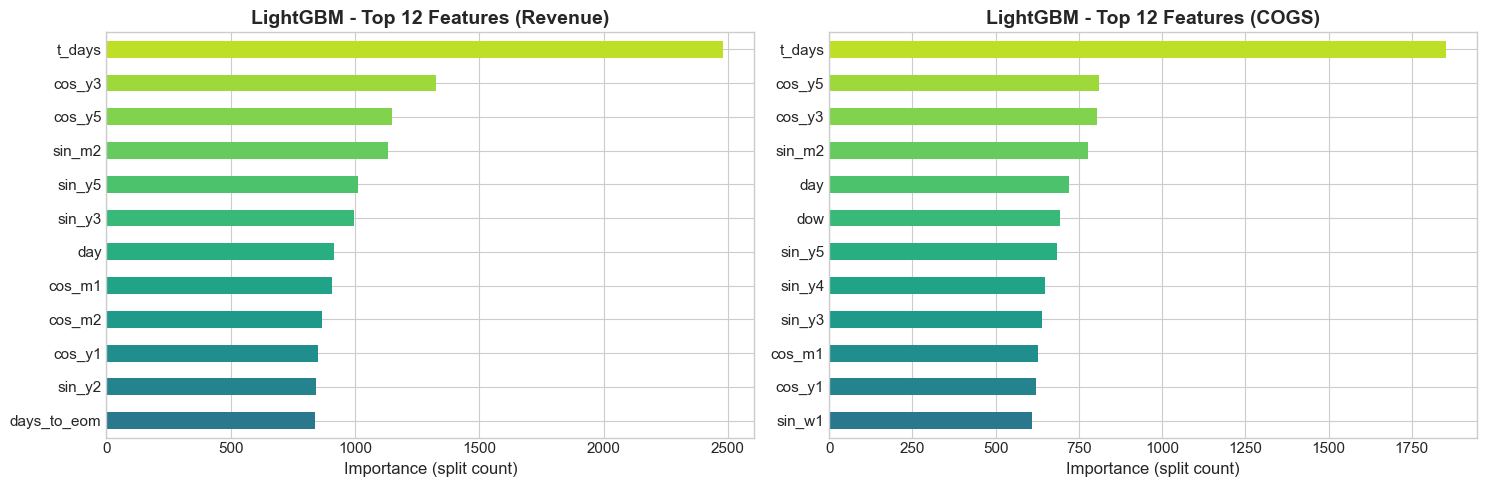
\includegraphics[width=\linewidth]{feature_importance.png}
  \caption{\textit{Đóng góp đặc trưng của mô hình LightGBM lõi.}}
  \label{fig:feat_imp}
\end{figure}

\textbf{Insight từ mô hình:} Biểu đồ Phân nhánh minh chứng chiến lược \textit{Lag-free} đã thành công rực rỡ. Nút gốc \texttt{t\_days} định hình xu hướng vĩ mô (Trend), trong khi các đặc trưng lượng giác Fourier (\texttt{cos\_y, sin\_y}) và đếm ngược sự kiện (\texttt{tet\_days\_diff}) đóng góp lượng chia nhánh cao nhất để định hình các đỉnh doanh thu.
\subsection{Hậu xử lý (Calibration)}
Toàn bộ quá trình huấn luyện diễn ra trên không gian Log (\textit{Log-space}) để trị nhiễu và sai phân phương sai. Trước khi xuất kết quả cuối cùng, hệ số điều chỉnh CR (Revenue) và CC (COGS) được nội suy thông qua kiểm định tương đối, bẻ dự báo về \textit{Level-space} để khắc phục hiện tượng \textit{Calibration Bias} (dự đoán thấp hơn thực tế của hàm hàm Log).

\newpage
\appendix
\section*{Phụ lục}
\section{ML}
\label{app:ML}
\begin{figure}[H]
  \centering
  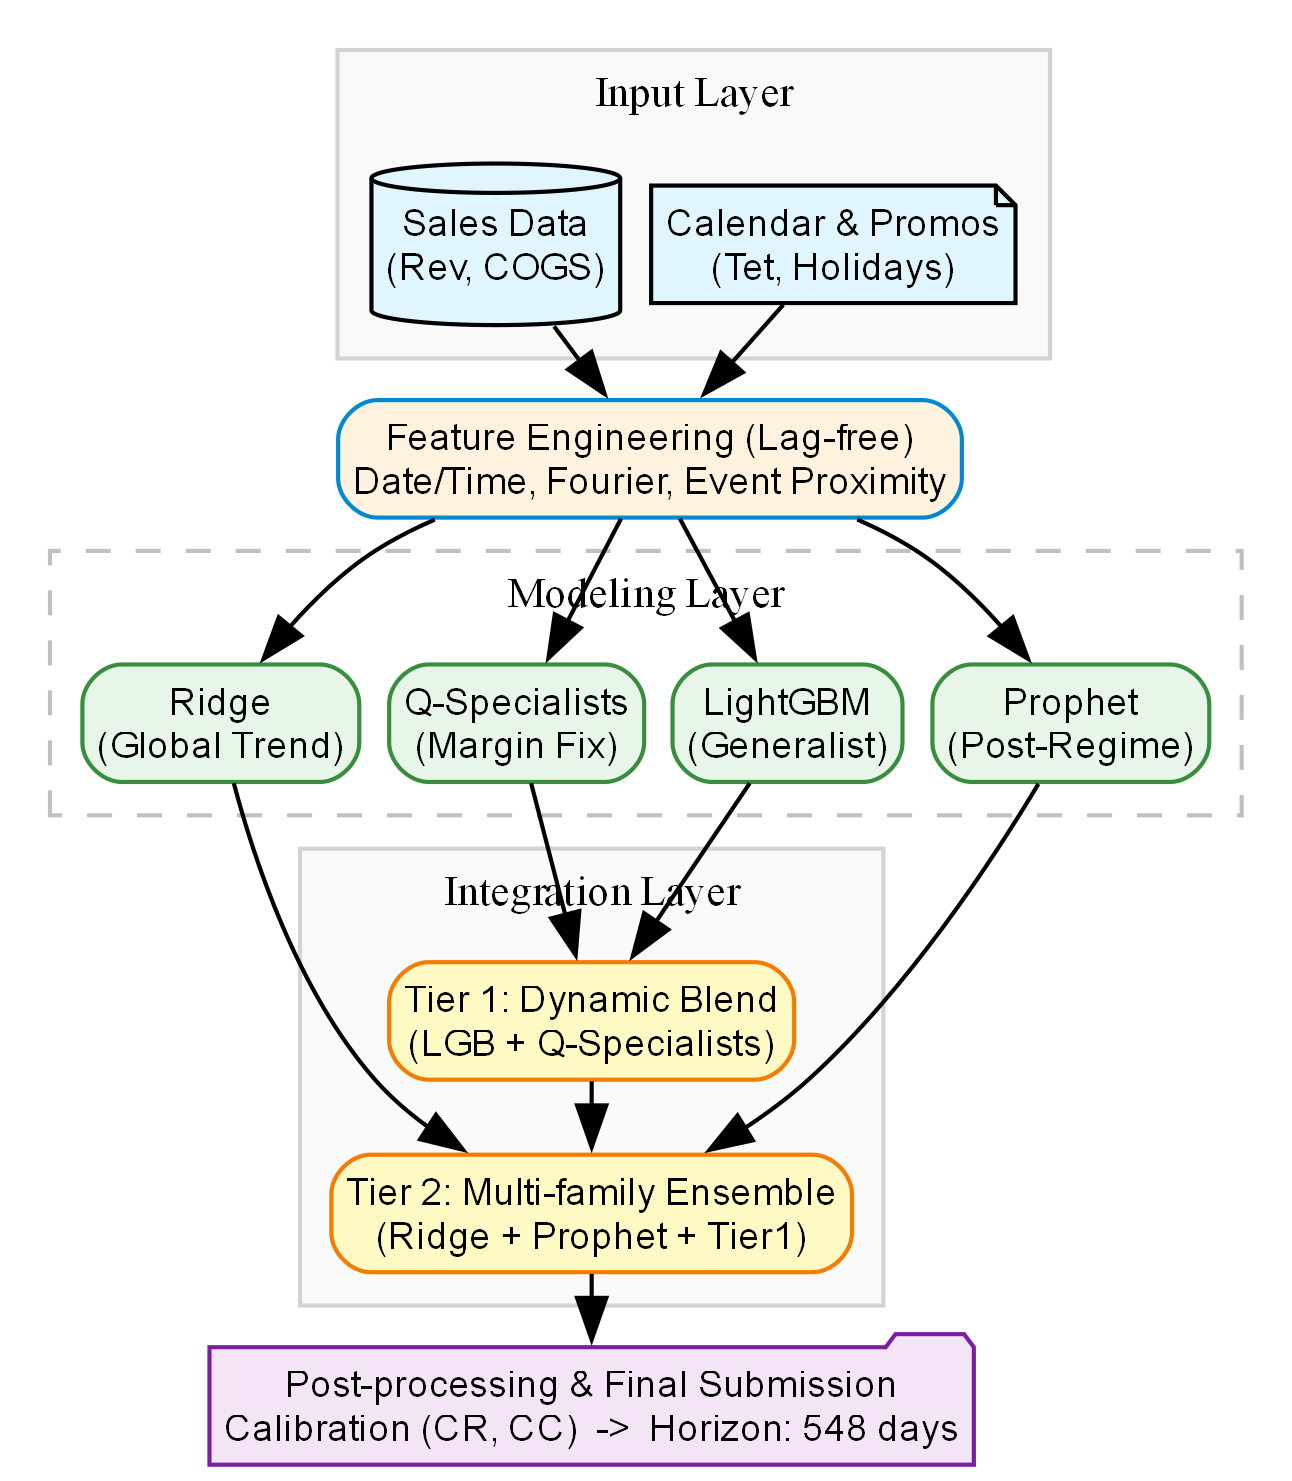
\includegraphics[width=\linewidth]{architecture.png}
  \caption{\textit{Luồng tích hợp dữ liệu và Kiến trúc 2 tầng.}}
  \label{fig:app:architecture}
\end{figure}
\subsection{Revenue, COGS, Profit}
\label{app: Revenue, COGS, Profit plot}
\begin{figure}[H]
  \centering
  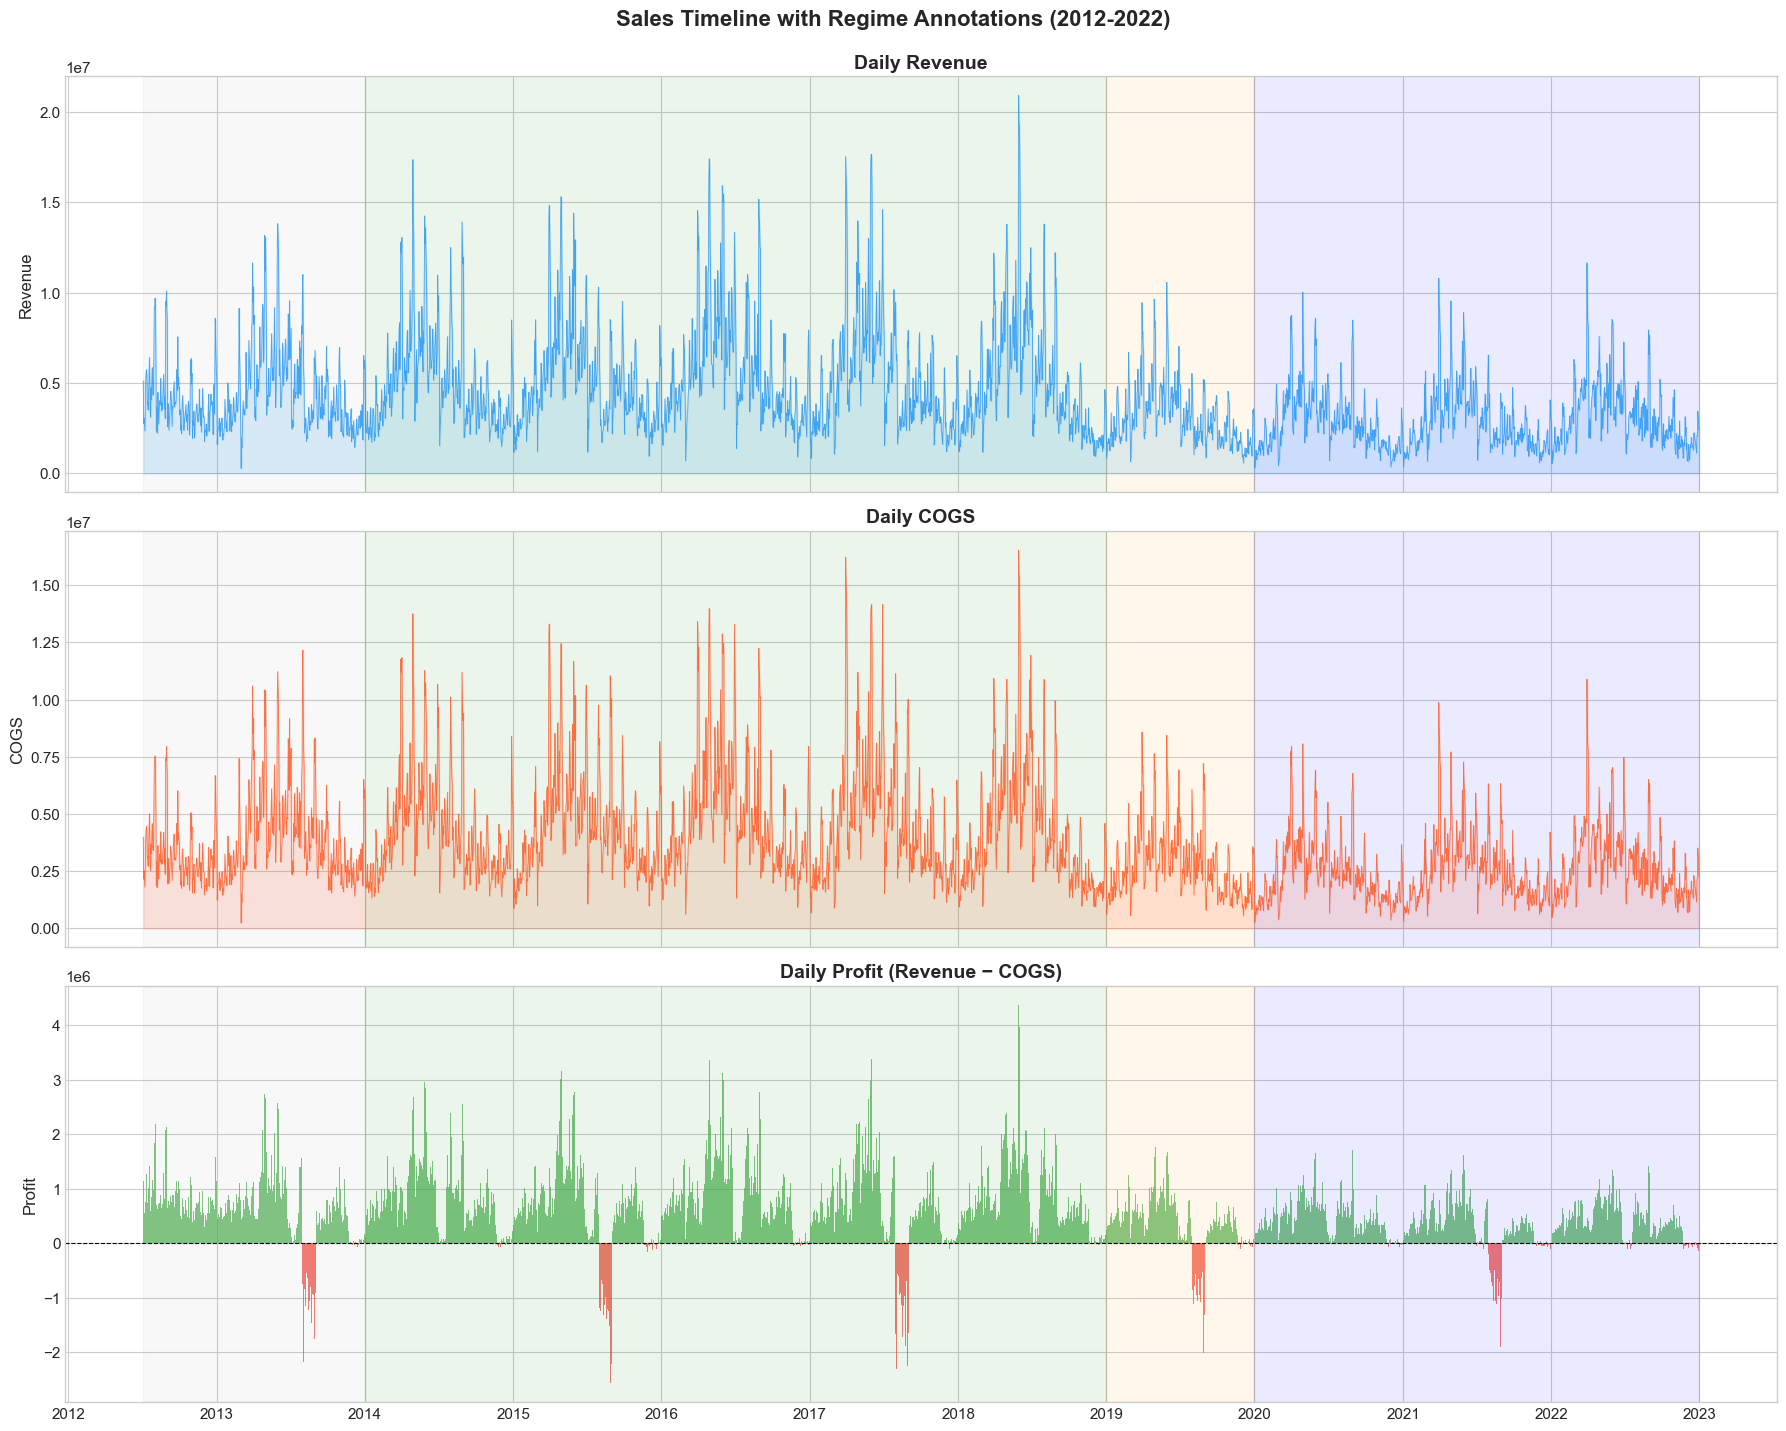
\includegraphics[width=\linewidth]{Revenue and COGS plot.png}
  \caption{\textit{Biểu đồ Revenue, COGS và Profit}}
  \label{fig:app:Revenue plot}
\end{figure}
\subsection{Thiết lập Pha trộn chuyên gia (Seasonal Blending Logic)}
\label{app: ML blending Logic}
Việc tối ưu hóa hệ số $\alpha$ tại Tier 1 đóng vai trò quyết định trong việc cân bằng giữa Rủi ro học vẹt (Overfitting) và Thiếu khớp (Underfitting). Hàm mục tiêu (Objective Function) để tối thiểu hóa RMSE kết hợp được biểu diễn như sau:
\begin{equation}
  \min_{\alpha} \sqrt{\frac{1}{N} \sum_{i=1}^{N} \left( y_i - \left[ (1 - \alpha_{q(i)}) \cdot \hat{y}_{base}^{(i)} + \alpha_{q(i)} \cdot \hat{y}_{spec}^{(i)} \right] \right)^2}
\end{equation}
Trong đó $q(i) \in \{1, 2, 3, 4\}$ tương ứng với quý của quan sát $i$. Dựa trên hiện tượng Base Model hoạt động xuất sắc tại Q1, Q2, Q4 trên tập validation, việc để thuật toán tối ưu tự do có thể vô tình triệt tiêu tính đa dạng của Ensemble (đẩy $\alpha \to 0$). Do đó, nhóm sử dụng chiến lược \textbf{Heuristic Hard-weights}, gán $\alpha_{1,2,4} = 0.6$ nhằm giữ vững tiếng nói của Base, và đẩy $\alpha_3 = 1.0$ để ủy quyền tuyệt đối cho Q3-Specialist xử lý các ngoại lệ margin phức tạp.
\subsection{Kiểm định và Chống Rò rỉ dữ liệu (Anti-Leakage Strategy)}
\label{app: ML Anti-Leakage Strategy}
Đặc thù của dữ liệu chuỗi thời gian bán lẻ đòi hỏi việc đánh giá phải mô phỏng chính xác quá trình luân chuyển thời gian trong thực tế. Các phương pháp Cross-Validation ngẫu nhiên (như K-Fold) bị loại bỏ hoàn toàn do vi phạm nguyên tắc nhân quả(Future-looking leakage).\\
Thay vào đó, hệ thống áp dụng chiến lược \textbf{3 Temporal Folds} (Kiểm định cuộn theo thời gian). Tại mỗi Fold $k$, mô hình chỉ được huấn luyện trên dữ liệu $T_{train} \le t_k$ và kiểm định trên $T_{val} > t_k$. Việc nghiêm ngặt không sử dụng Lag Features đảm bảo sai số (nếu có) được cô lập tại các thời điểm cục bộ, không lây lan theo hiệu ứng "quả cầu tuyết" sang các phiên dự báo dài hạn (18 tháng).
\subsection{Tối ưu trọng số Ensemble bằng NNLS (Non-Negative Least Squares)}
\label{app: ML NNLS}
Tại Tier 2, bài toán kết hợp kết quả từ các mô hình độc lập (Ridge, Prophet, Tier 1) được định hình dưới dạng tối ưu hóa bình phương tối thiểu có ràng buộc không âm (NNLS). Giả sử $X \in \mathbb{R}^{N \times M}$ là ma trận chứa dự báo của $M$ mô hình trên $N$ điểm dữ liệu validation, và $y \in \mathbb{R}^N$ là nhãn thực tế. Trọng số kết hợp $w$ được tìm ra bằng cách giải bài toán NNLS:
\begin{equation}
  \min_{w} \left\| y - Xw \right\|_2^2 \quad \text{s.t.} \quad w_m \ge 0, \forall m \in \{1, \dots, M\}
\end{equation}
Việc ép buộc trọng số $w \ge 0$ mang lại hai lợi thế cốt lõi: (1) Ngăn chặn hiện tượng âm hóa trọng số (\textit{negative weights}) khi các mô hình thành phần có tính cộng tuyến (collinearity) cao; (2) Đảm bảo dự báo cuối cùng luôn nằm trong bao lồi (\textit{convex hull}) của các mô hình gốc. Điều này giúp hệ thống tránh được các ngoại suy cực đoan (extreme extrapolations), từ đó duy trì tính ổn định (robustness) trên tập Test bí mật.
\section{Chart 4}
\label{app:chart4}
\begin{figure}[H]
  \centering
  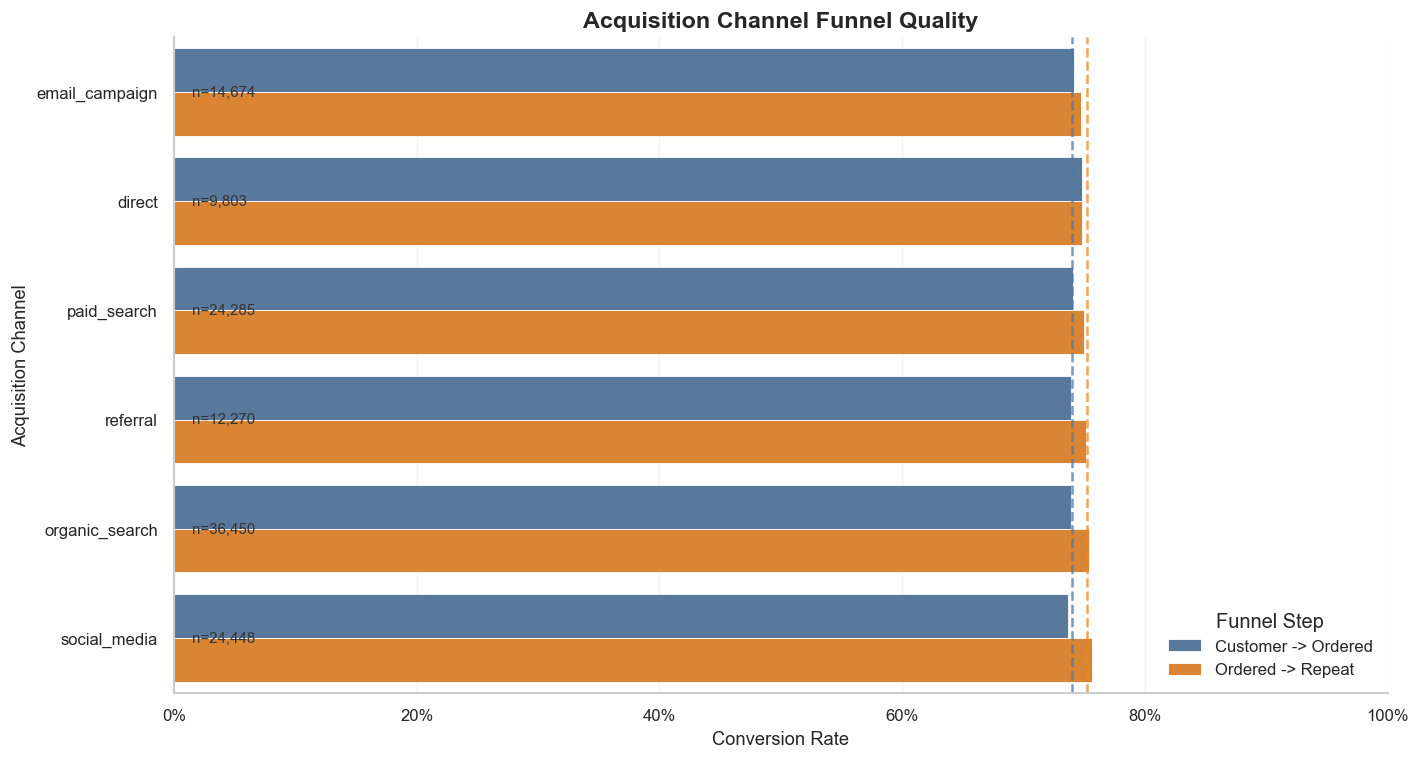
\includegraphics[width=\linewidth]{Chart4.png}
  \caption{\textit{Tỉ lệ mua lại theo kênh truyền thông}}
  \label{fig:app:demand_by_channel}
\end{figure}
Chart 4 cho thấy chất lượng demand giữa các kênh khá sát nhau, nên bài toán không phải chọn một kênh thắng tuyệt đối mà là hiểu kênh nào tạo ra base khách đủ lớn và ổn định hơn.\\
Hai tỷ lệ chính (Customer -> Ordered và Ordered -> Repeat) dao động trong biên độ hẹp giữa các kênh.\\
\textbf{Direct} nhỉnh hơn ở activation, \textbf{Social Media} nhỉnh nhẹ ở repeat nhưng chưa có kênh nào vượt trội tuyệt đối.\\
Khi chênh lệch tỷ lệ nhỏ, quy mô khách của từng kênh mới là yếu tố quyết định tác động doanh thu thực tế.\\
Ưu tiên kênh có volume lớn và hiệu quả ổn định, đồng thời tối ưu trải nghiệm sau mua thay vì kỳ vọng thay đổi lớn chỉ từ việc đổi kênh acquisition.
\newpage
\bibliographystyle{plainnat}
\bibliography{ref}
\end{document}
